\section{Bedienung des Rastertunnelmikroskops}\label{sec:versuch}
Bei der Versuchsdurchführung wird ein RTM mit einem externen Controller und der zugehörigen Software \texttt{Easyscan 2} verwendet.
Der Experimentierplatz ist in \cref{fig:versuchsplatz} gezeigt.
\begin{figure}[H]
	\centering
	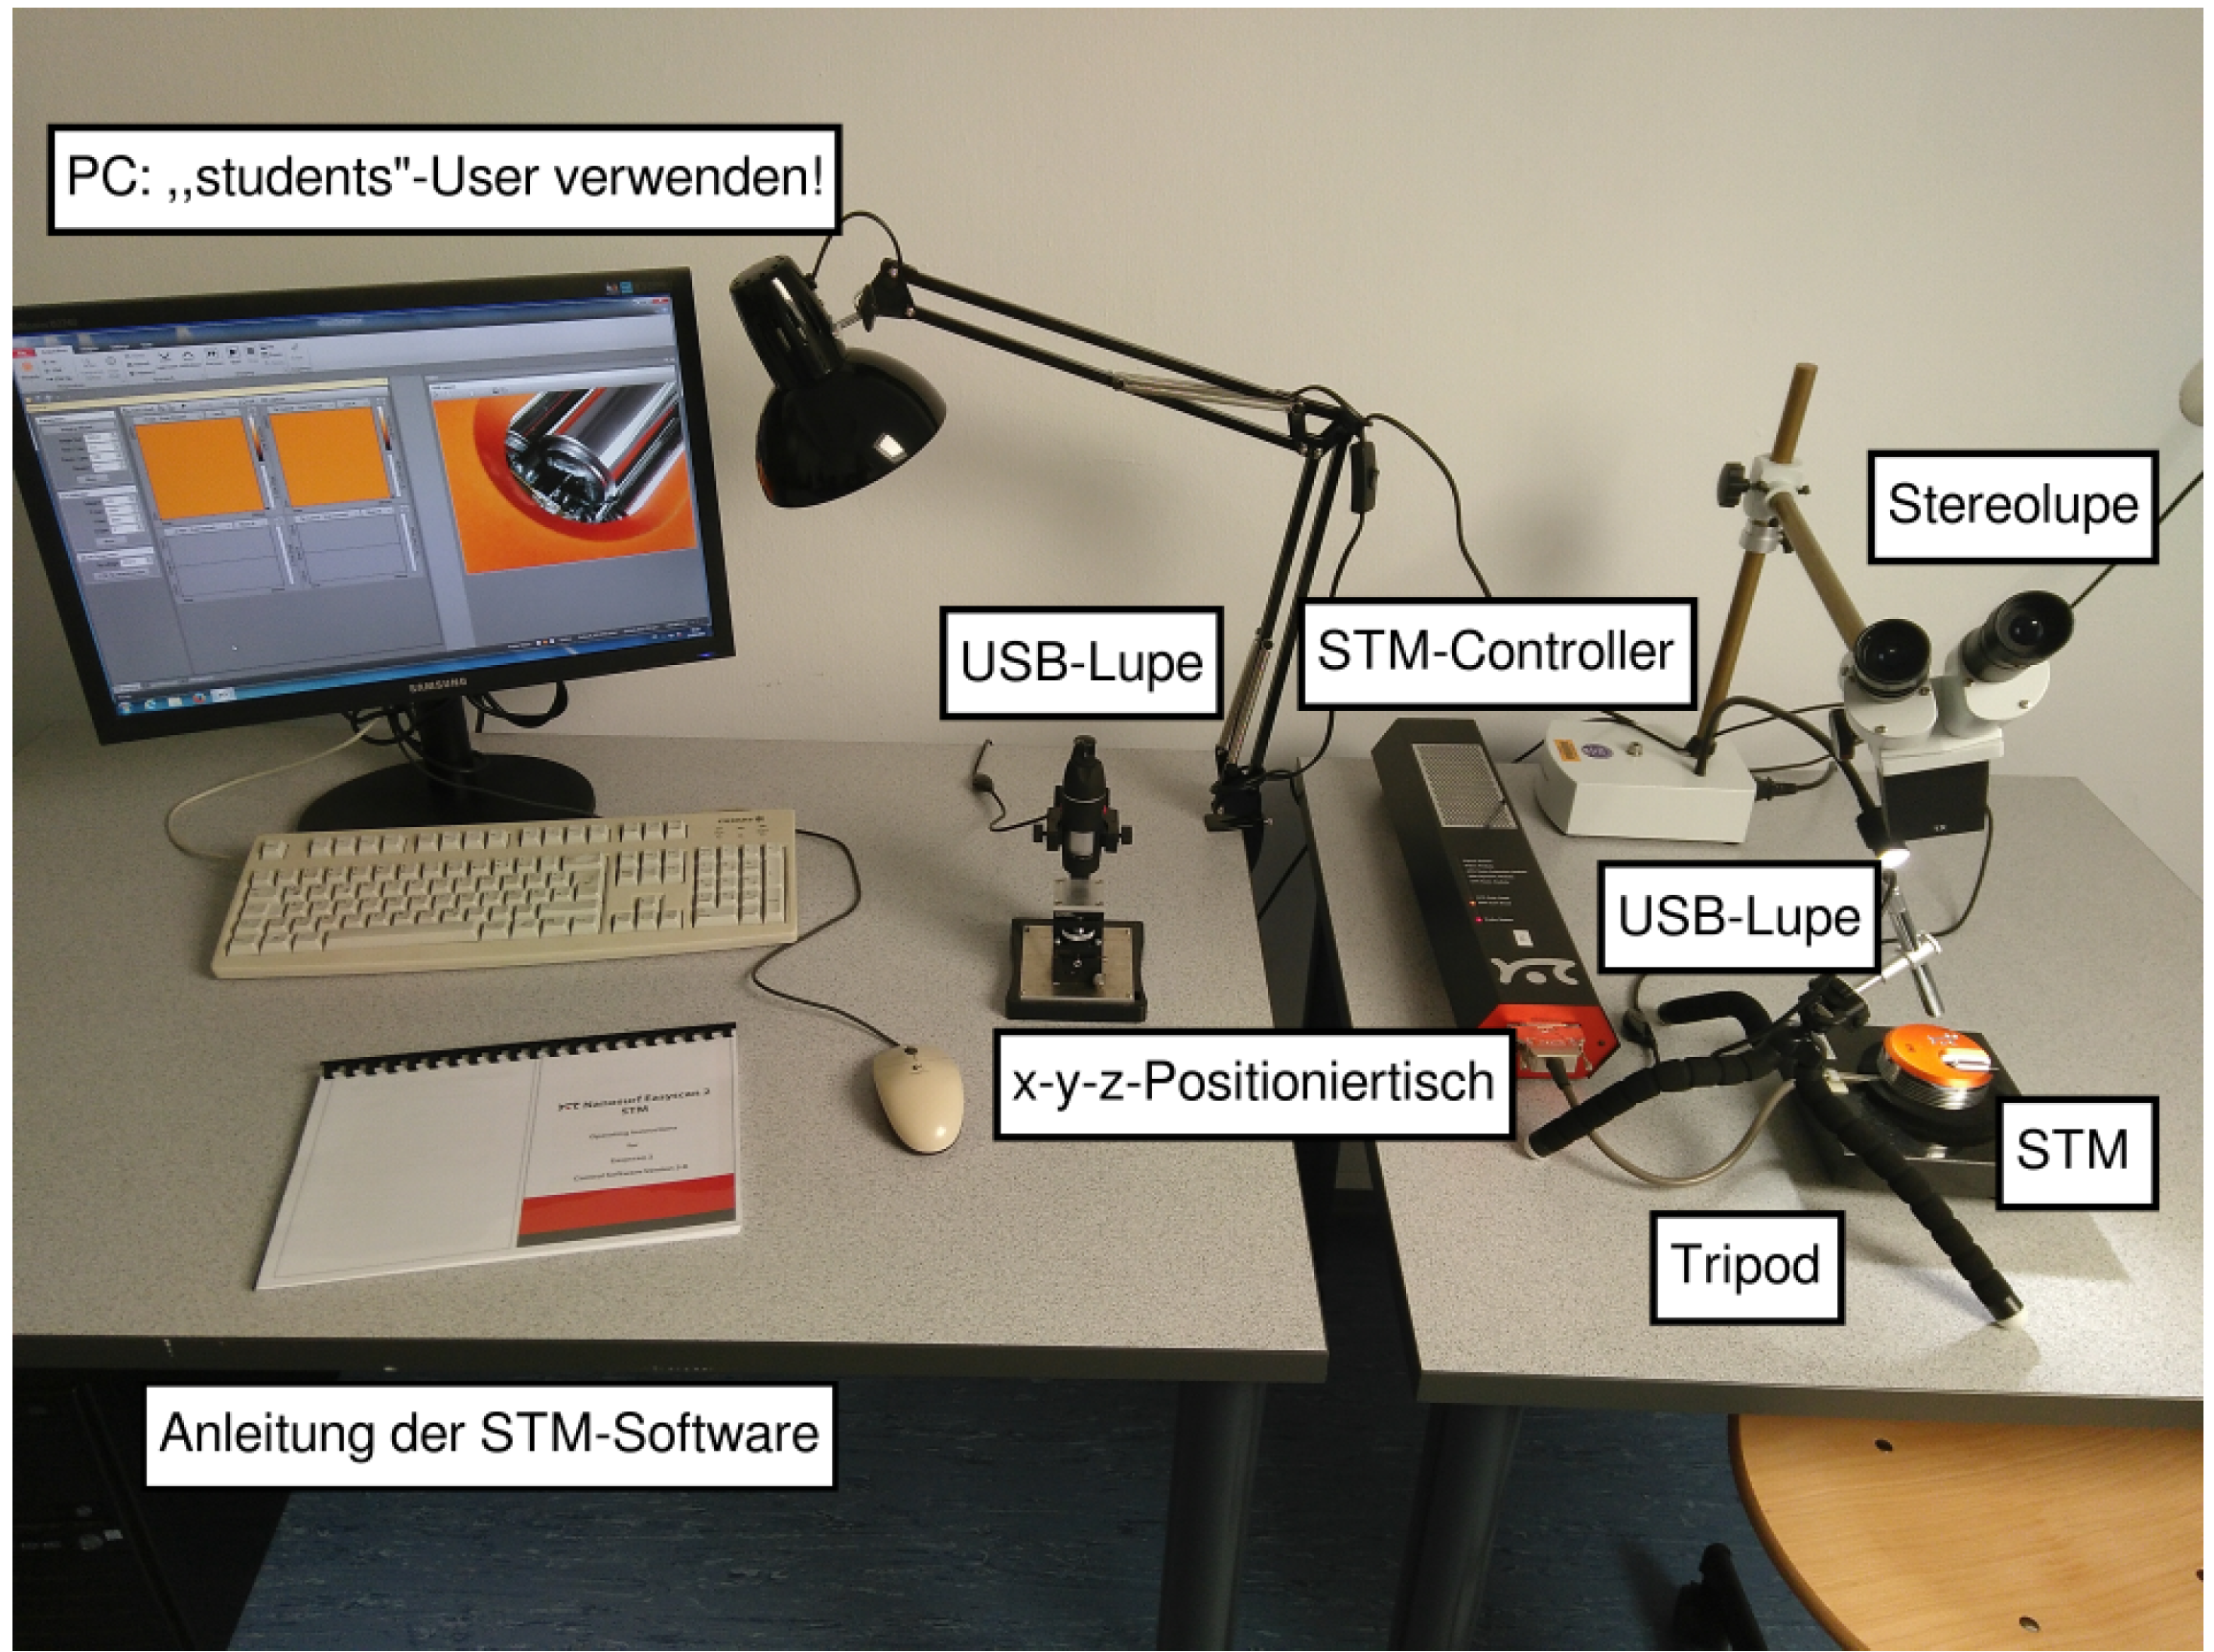
\includegraphics[width=0.8\linewidth]{../figs/versuchsplatz.png}
	\caption{Experimentierplatz mit RTM und dem notwendigen Zubehör (Quelle: \cite{skript})}
	\label{fig:versuchsplatz}
\end{figure}
Um mit dem RTM arbeiten zu können, wird der RTM-Controller über einen Kippschalter eingeschaltet. Anschließend wird der beistehende Rechner
hochgefahren, um die für den RTM-Controller benötigte Software \texttt{Easyscan 2} zu öffnen. Außerdem ist der Arbeitsbereich mit den Eingabegeräten
des Rechners (Tastatur und Maus) auf einem anderen Tisch als das RTM platziert, sodass die vielen Berührungspunkte der Hände, Arme, Füße und Beine mit dem Tisch während der Bedienung
der Software keinen Einfluss auf die Arbeitsweise des RTMs haben. Ohnehin ist das RTM auf einem schwingungsdämpfenden Körper befestigt, um
den Einfluss von Vibrationen auf die Messungen zu verringern, allerdings hat sich bei der Versuchsdurchführung tatsächlich gezeigt, dass leichte Zusammenstöße
mit dem RTM-Tisch zu kurzzeitigen Ausreißern während eines Messprozesses führen, weshalb eine Aufteilung der beteiligten Arbeitsgeräte definitv sinnvoll ist.\par
Auf dem Tisch mit dem Rechner ist zudem eine USB-Lupe positioniert, mit der die verwendeten Proben und Spitzen auf ihre Qualität untersucht werden können.
Für diese USB-Lupe wird eine separate Software verwendet.\par
Das RTM weißt eine Öffnung auf, in welche die Spitze und Probe eingesetzt werden können. Diese Öffnung ist mit einer Schutzkappe abgedeckt, welche aber für
die Versuchsdurchführung entfernt werden kann. Darüber hinaus wird eine weitere USB-Lupe (montiert auf einem Dreibein) auf die Öffnung des RTMs gerichtet,
um später die Annäherung der Probe an die Spitze beobachten zu können. Das resultierende Bild dieser USB-Lupe kann in \texttt{Easyscan 2} dargestellt werden.\par
Die Proben, der Spitzendraht und das benötigte Zubehör befindet sich in einer Box (siehe \cref{fig:koffer}). Wenn eine bestimmte Probe untersucht werden soll,
wird zunächst der Probenhalter mit Isopropanol gereinigt. Ebenso wird die Rückseite der Probe mit Isopropanol gereinigt, bevor sie mit der Probenpinzette
auf dem Probenhalter magnetisch befestigt wird. Vor einer Messung wird immer die zu untersuchende Probe unter der USB-Lupe betrachtet. Die Messspitze wird mit einem
Seitenschneider aus einem Platin-Iridium-Draht zugeschnitten. Die angefertigte Messspitze wird ebenfalls unter der USB-Lupe auf ihre grobe Qualität hin betrachtet.
Um die Spitze handzuhaben, wird eine Spitzenpinzette benutzt. Um eine Spitze unter der USB-Lupe zu untersuchen, kann diese in einem separaten RTM-Innenleben befestigt werden.\par
Nun kann die angefertigte Messspitze in dem RTM befestigt werden. Anschließend kann der Probenhalter mit der zu untersuchenden Probe auf die Kontaktstellen
des \textit{Stick-Slip}-Piezos gelegt werden.
\begin{figure}[H]
	\centering
	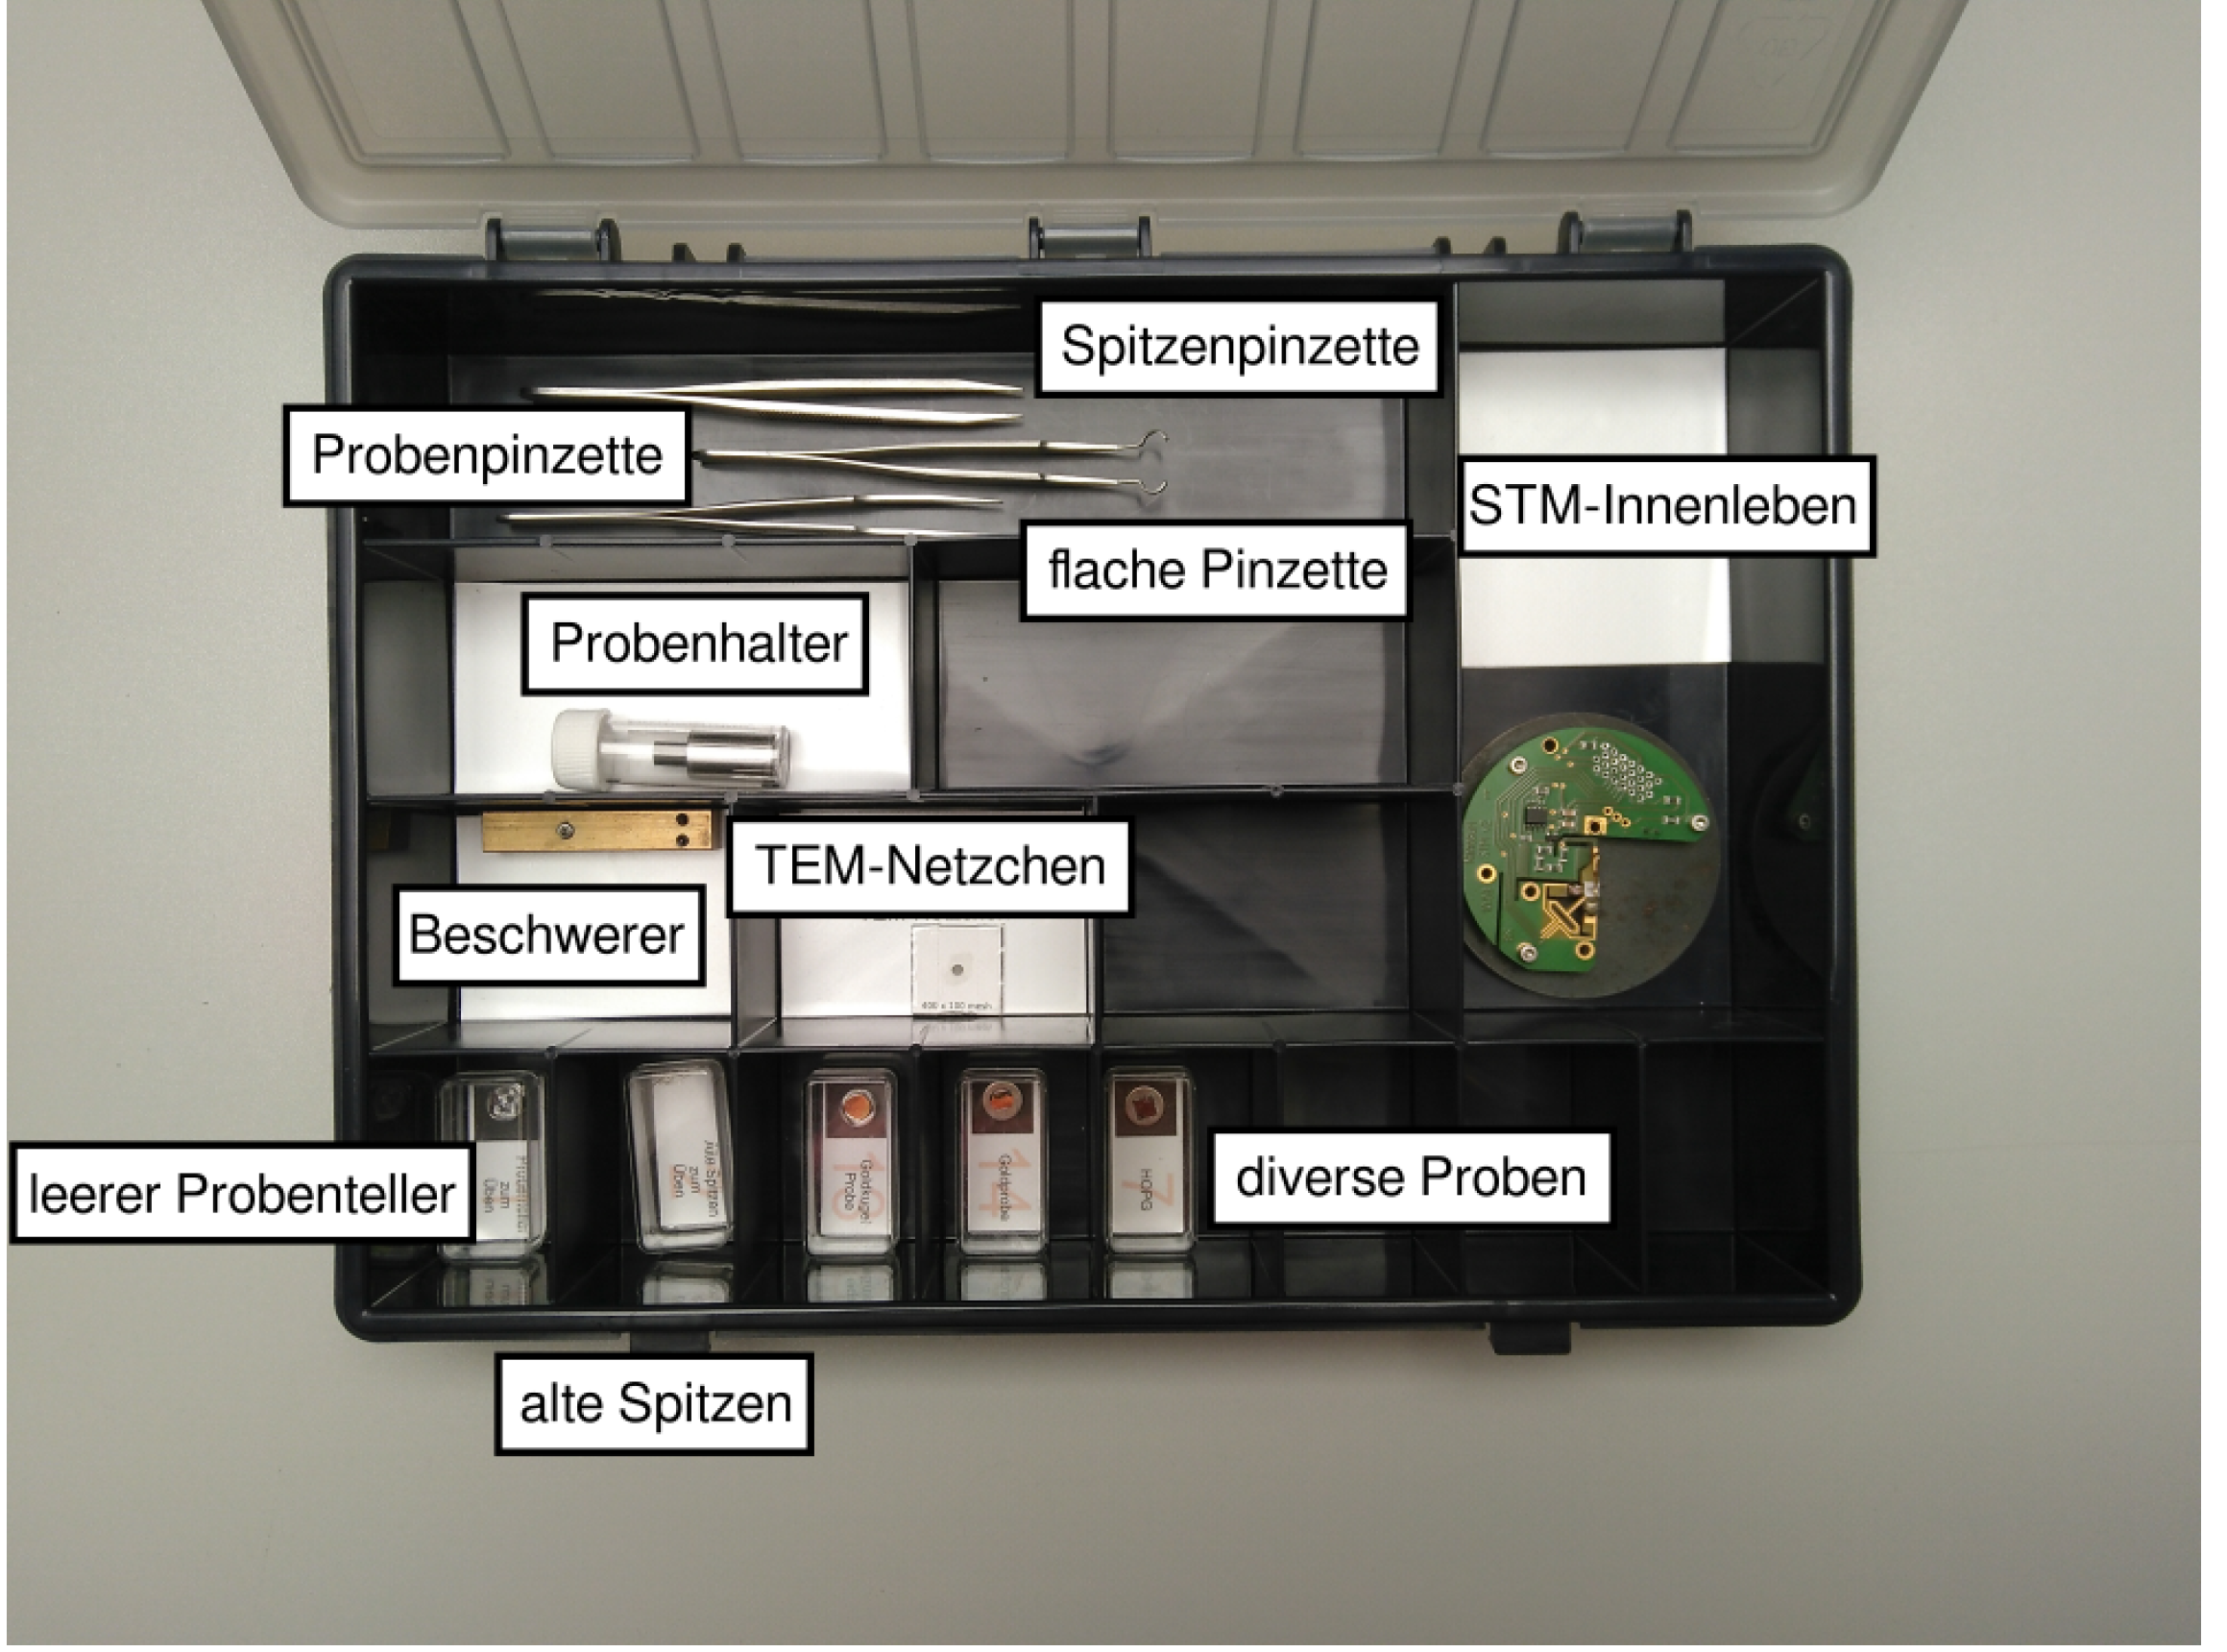
\includegraphics[width=0.8\linewidth]{../figs/koffer.png}
	\caption{Box mit den Proben und dem benötigten Zubehör (Quelle: \cite{skript})}
	\label{fig:koffer}
\end{figure} Da der zu messende Tunnelstrom exponentiell mit dem Abstand zwischen Spitze und Probe abnimmt, ist es für die Arbeitsweise des RTMs notwendig,
den Abstand zwischen Spitze und Probe auf etwa einen Atomdurchmesser (\SI{0,1}{\nano \meter}) einzustellen. Um dies technisch zu ermöglichen, wird der
\textit{Stick-Slip}-Piezo benötigt. Ein piezoelektrisches Stellelement verformt sich unter Anlegung einer Spannung, da die Ladungsschwerpunkte
gegeneinander verschoben werden. Da diese physischen Verformungen auf sehr kleinen Längenskalen stattfinden, sind mit Piezos feine Bewegungen im sub-\unit{\nano \meter}-Bereich
möglich. Bei Benutzung des \textit{Stick-Slip}-Piezos wird eine Sägezahnspannung an dieses angelegt, sodass der Probenhalter zunächst um eine kleine Distanz
verschoben werden kann (zur Spitze hin oder von der Spitze weg). Hier haftet der Probenhalter aufgrund der Haftreibung an den Kontaktstellen des Piezos.
Zudem wird ein Beschwerer auf den Probenhalter gelegt, damit die Funktionsweise des \textit{Stick-Slip}-Antriebs verbessert wird.
Dann bewegt sich das Piezo ruckartig in die entgegengesetzte Richtung, wobei aber der Probenhalter (inklusive Beschwerer) aufgrund seiner Trägheit seine Position nicht verändert.
Da sich dieser Prozess mit der angelegten Sägezahnspannung periodisch wiederholen lässt, kann der Probenhalter gleichzeitig fein und über größere Distanzen bewegt werden.\par
Um die Probe an die Spitze anzunähern, wird in der Software zunächst die Funktion \textit{Advance} benutzt. Damit wird die Probe manuell möglichst nah an die Spitze
herangefahren. Sobald unter der USB-Lupe über dem RTM kein Abstand mehr zwischen Spitze und Probe zu erkennen ist, wird die Funktion \textit{Approach} benutzt.
Mit dieser Funktion wird die Probe automatisch in möglichst feinen Abständen an die Spitze herangefahren. Dieser Annäherungsprozess endet, sobald ein Tunnelstrom messbar wird.
Soll die Probe später von der Spitze entfernt werden, wird zunächst die Funktion \textit{Withdraw} (Zurückfahren in feinen Abständen) und dann die Funktion
\textit{Retract} (grobes Entfernen der Probe von der Spitze) benutzt.\par
Die Spitze wird über insgesamt drei Piezoelemente bewegt. Eines dieser Piezoelemente dient zur feinen Änderung der Höhe der Spitze über der Probenoberfläche.
Die anderen beiden Piezoelemente dienen zur Rasterbewegung der Spitze. Hier kann die Rastergeschwindigkeit manuell eingestellt werden.
Ebenso lässt sich die Spannung zwischen Spitze und Probe manuell einstellen. Soll nun die zu untersuchende Oberfläche abgerastert werden, stehen im wesentlichen zwei
Betriebsmodi (\textit{constant-current-mode} und \textit{constant-height-mode}) zur Verfügung.\par
Bei dem \textit{constant-current-mode} arbeitet das RTM so, dass der zu messende Tunnelstrom konstant gehalten wird. Dafür muss laufend die Höhe der Spitze
über der Probenoberfläche geändert werden. Um auf diese Änderungen zu reagieren, arbeitet das RTM mit einem Regelkreis. Im wesentlichen wird dem Regelkreis
ein Strom-Sollwert vorgegeben, wodurch mit dem Strom-Istwert eine Fehlerfunktion berechnet wird. Bei diesem Versuch wird ein PI-Regelkreis (\textit{Proportional-Integral}) verwendet,
wobei das \textit{Proportional}-Glied eine zu der Fehlerfunktion proportionale Stellgröße berechnet und das \textit{Integral}-Glied die Fehlerfunktion über eine gewisse
Integrationszeit integriert. Um das RTM im \textit{constant-current-mode} zu betreiben, werden die Parameter für P und I entsprechend groß gewählt (z.B. $\mathrm{P} = 1000$ und $\mathrm{I} = 2000$),
sodass auf rasche Änderungen möglichst schnell reagiert werden kann. Dieser Betriebsmodus sollte bei einer ersten Messung einer Probe verwendet werden, da hier verhindert wird,
dass die Spitze in die Probe reinfährt.\par
Im \textit{constant-height-mode} wird der Regelkreis prinzipiell nicht benötigt, da die Höhe der Spitze über der Probenoberfläche konstant gehalten werden soll.
Damit werden hier Paramter für P und I nahe null gewählt. Dieser Betriebsmodus sollte erst dann gewählt werden, wenn ein möglichst flacher Bereich der Probenoberfläche abgerastert wird,
sodass die Spitze nicht in die Probe gefahren wird.\par
Mithilfe von \texttt{Easyscan 2} kann der gewünschte abzurasternde Bereich auf der Probenoberfläche ausgewählt werden. Für eine gelungene Messung müssen häufig Parameter wie Spannung
und Rastergeschwindigkeit variiert werden.